\chapter{Adatbázisfüggvények}
\thispagestyle{empty}

Adatbázisfüggvények segítségével számításokat
végezhetünk az adattábla értékeivel egy dinamikusan
változtatható keresési tartomány feltételei alapján. Az
irányított szűrőhöz hasonlóan e tartomány egy
sorának cellái között ÉS logikai kapcsolat lesz, a sorok
között pedig VAGY. Minden adatbázisfüggvénynek három
argumentuma van: \textbf{adatbázis}, \textbf{adatbázismező}
és \textbf{keresési feltétel}.

Az első magát az adattáblát adja meg. Az irányított
szűrő tulajdonságait bemutató példánál ez az A1:E17
tartomány (\ref{SzűrésEredmények} ábra).

A \textbf{keresési feltétel} a feltételeket tartalmazó
cellatartomány. \Aref{SzűrésEredmények} ábrán a A22:E24.
Ebben a tartományban csak akkor használhatunk reguláris
kifejezéseket ha bekapcsoljuk az
\textbf{Eszközök --  Beállítások --  OpenOffice.org Calc --
Számítás} panelen a \textbf{Reguláris kifejezések
engedélyezése képletekben} kapcsolót.

Az \textbf{adatbázismező} annak az oszlopnak a sorszáma az
adattáblán beül, amelyikben a függvény működni fog. A 0
értékkel megadhatjuk a teljes adattartományt. Mezőnevet is
megadhatunk idézőjelek közé írva.


\Aref{AdatbázisFüggvények} táblázat a gyakrabban használt
adatbázisfüggvényeket mutatja.

\begin{table}[!h]
\begin{center}
\caption{Gyakrabban használt adatbázisfüggvények}\label{AdatbázisFüggvények}
\begin{tabular}{|m{2.5cm}|m{8cm}|}
\hline
DSUM &
A keresési feltételeknek megfelelő cellák összegét
számítja ki.\\ \hline
DMAX &
A keresési feltételeknek megfelelő cellák közül a
legnagyobb értéket adja vissza.\\ \hline
DMIN &
A keresési feltételeknek megfelelő cellák közül a
legkisebb értéket adja vissza.\\ \hline
DAVERAGE &
A keresési feltételeknek megfelelő cellák átlagát
számítja ki.\\ \hline
DCOUNT &
Megszámolja a számokat tartalmazó rekordokat az adattáblában,
amelyek megfelelnek a keresési feltételeknek.\\ \hline
DCOUNTA &
Megszámolja a számokat és szöveget tartalmazó rekordokat az
adattáblában, amelyek megfelelnek a keresési
feltételeknek.\\ \hline
\end{tabular}
\end{center}
\end{table}

\clearpage
\section{26. feladat}
{\itshape
Számítsuk ki adatbázisfüggvények felhasználásával \aref{IrányítottSzűrő} 
ábrán látható feltételeknek megfelelő rekordok:}

{\itshape
a) darabszámát}

{\itshape
b) készletszámok összegét}

{\itshape
c) a legnagyobb beszerzési árat }

{\itshape
d) a legkisebb beszerzési árat}

{\itshape
e) a beszerzési árak átlagát}

{\itshape
Módosítsuk a keresési feltételeket, hogy a K betűvel
kezdődő, 10~000~Ft-nál kisebb beszerzési árú
 rekordokat határozza meg.}

A szűrő kikapcsolása után másoljuk az A1:E24 tartományt
egy üres munkalapra. A Reguláris kifejezések engedélyezése
képletekben kapcsolót a Beállítások ablakban kapcsoljuk be.
Az A26:A30 tartományba írjuk \aref{26-feladat} ábrán látható
tartalmakat és adatbázisfüggvények segítségével
számítsuk ki a C26:C30 tartomány celláit. A rekordok
számának meghatározásánál használhatjuk a DCOUNTA
függvényt. Olyan mezőt válasszunk második argumentumnak,
amelyiket az adattábla módosításánál is mindenképp
kitöltünk. Esetünkben ilyen lehet az első, a Kód mező.

\begin{figure}[!h]
\begin{center}
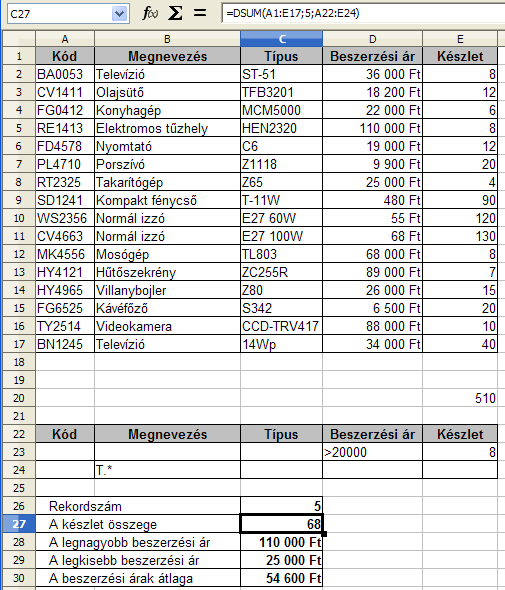
\includegraphics[width=12.36cm]{oocalcv1-img120.png}
\caption{26. feladat}\label{26-feladat}
\end{center}
\end{figure}

A készlet összegének kiszámításának képletét látjuk
\aref{26-feladat} ábrán. A további három függvény argumentuma ugyanaz
lesz: \textsf{\textbf{\textcolor{black}{(A1:E17;4;A22:E24)}}}, a
használt függvények pedig DMAX, DMIN és DAVERAGE. Az első
két eredményt leellenőrizhetjük, összehasonlítva az
Irányított szűrő példájában kapottakkal. A SUBTOTAL
függvény ott ugyanúgy a készletszámok összegét
határozta meg, ugyanazokkal a keresési feltételekkel.

Módosítsuk a keresési feltételeket, és az
adatbázisfüggvények az új feltételeknek megfelelő
rekordok alapján határozzák meg értékeket (\ref{26-feladatEredmény} ábra).

\begin{figure}[!h]
\begin{center}
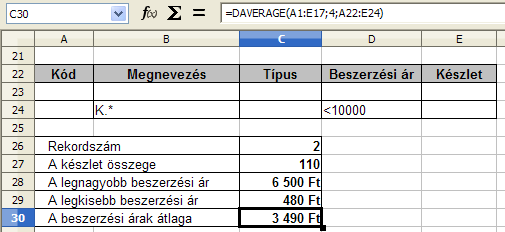
\includegraphics[width=12.36cm]{oocalcv1-img121.png}
\caption{26. feladat --  eredmény}\label{26-feladatEredmény}
\end{center}
\end{figure}

Az ebben a fejezetben tárgyalt függvények \aref{13-fejezetFüggvények}
táblázatban láthatóak.

\begin{table}[!h]
\begin{center}
\caption{A fejezetben tárgyalt függvények}\label{13-fejezetFüggvények}
\begin{tabular}{|m{3cm}|m{8cm}|m{3cm}|}
\hline
 & & \multicolumn{1}{c|}{\textbf{Megfelelője a}} \\
\multicolumn{1}{|c|}{\textbf{A függvény}}&
\multicolumn{1}{c|}{\textbf{Funkciója}}&
\multicolumn{1}{c|}{\textbf{magyar}} \\
\multicolumn{1}{|c|}{\textbf{neve}} & &
\multicolumn{1}{c|}{\textbf{Microsoft}} \\
 & & \multicolumn{1}{c|}{\textbf{Excelben}} \\
\hline
DSUM & A keresési feltételeknek megfelelő cellák összegét
számítja ki. & AB.SZUM\\ \hline
DMAX & A keresési feltételeknek megfelelő cellák közül a
legnagyobbat értéket adja vissza. & AB.MAX\\ \hline
DMIN & A keresési feltételeknek megfelelő cellák közül a
legkisebb értékét adja vissza. & AB.MIN\\ \hline
DAVERAGE & A keresési feltételeknek megfelelő cellák átlagát
számítja ki. & AB.ÁTLAG\\ \hline
DCOUNT & Megszámolja a számokat tartalmazó rekordokat az adattáblában,
amelyek megfelelnek a keresési feltételeknek. & AB.DARAB\\ \hline
DCOUNTA & Megszámolja a számokat és szöveget tartalmazó rekordokat az
adattáblában, amelyek megfelelnek a keresési feltételeknek. &
AB.DARAB2\\ \hline
\end{tabular}
\end{center}
\end{table}

